\section[Общесистемная часть]{ОБЩЕСИСТЕМНАЯ ЧАСТЬ}

\subsection{Описание объекта проектирования}

Объектом проектирования является мобильное приложение,
выполняющее учет и представление финансовых данных пользователя.

Ввод данных осуществляется пользователем либо вручную,
либо с помощью алгоритма распознавания данных с изображения,
полученного фотокамерой мобильного устройства.

Хранение данных осуществляется средствами мобильной платформы в
виде реляционной базы данных.

Вывод данных сводится к построению различных отчетов об изменении
баланса денежных средств за выбранный период.

\subsection{Постановка задачи проектирования}

Требуется выполнить проектирование автоматизированной системы,
выполненной в виде мобильного приложения и обладающей следующими
функциональными возможностями:
\begin{itemize}
\item ручной ввод финансовых данных с возможностью выбора счёта,
  валюты и категории;
\item автоматический ввод финансовых данных с изображения,
  содержащего некоторые числовые данные;
\item хранение финансовых данных в зашифрованном виде;
\item построение графиков изменения баланса денежных средств
  на выбранном счёте за выбранный период;
\item построение отчета о расходах пользователя
  за выбранный период с группировкой по категориям.
\end{itemize}

Разработанное приложение должно иметь простой и удобный
пользовательский интерфейс.

Оформление работы требуется выполнить в соответствии
со стандартом оформления курсовых и дипломных работ~\cite{stp2013}.

\pagebreak
\subsection{Концептуальная модель системы}

В целом, можно выделить следующие сценарии использования приложения:
\begin{itemize}
  \item ввод финансовых данных;
  \item просмотр отчетов на основании накопленных данных.
\end{itemize}

Эти сценарии приведены на рисунке~\ref{fig:use_cases}.

\begin{figure}[h!]
  \centering
  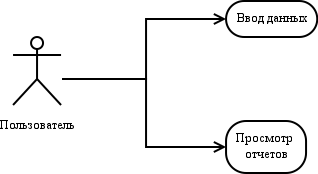
\includegraphics[width=92mm]{pic/use_cases}
  \caption{Диаграмма прецендентов \\ использования приложения}
  \label{fig:use_cases}
\end{figure}

Ввод финансовых данных предполагает ручной либо автоматический ввод
значения изменения суммы денежных средств определенной валюты
на определенном счёте и категории.
Просмотр отчётов предполагает выборку требуемой информации из базы
данных и её представление в желаемой форме.

Исходя из этого, можно выделить следующие сущности рассматриваемой
предметной области:
\begin{itemize}
\item счета;
\item категории;
\item изменения состояния счёта.
\end{itemize}

Эти сущности, а также связи между ними, приведены на рисунке~\ref{fig:entities}.

\begin{figure}[h!]
  \centering
  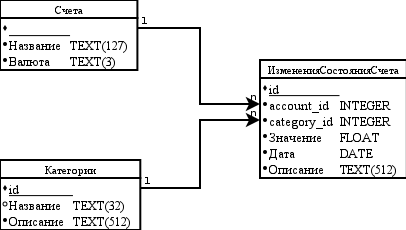
\includegraphics[width=150mm]{pic/entities}
  \caption{Основные сущности предметной области}
  \label{fig:entities}
\end{figure}

Сущность <<Счёт>> соответствует, платежной карте
и состоит из названия, идентификатора и валюты, в которой производятся расчёты.

Сущность <<Категория>> соответствует некоторой категории доходов или расходов
пользователя, например <<Расходы на еду>>, или <<Заработная плата>>
и состоит из названия, идентификатора и описания.

Сущность <<Изменение состояния счёта>> отражает изменение состояния счёта
пользователя и включает в себя идентификаторы счёта и категории,
значения изменения счёта, даты изменения и комментария.

Сущности <<Счёт>> и <<Изменение состояния счёта>> связаны связью
вида один-ко-многим, так как одному счёту может соответствовать
множество записей об изменении его состояния.

Подобным образом, сущности <<Категория>> и <<Изменение состояния счёта>>
также связаны связью вида один-ко-многим, поскольку
каждой категории прибылей и затрат может соответствовать множество
записей об изменении состояния счёта.